\documentclass{article}
\usepackage[utf8]{inputenc}
\usepackage{polski}
\usepackage{geometry}
\usepackage{pdfpages}
\usepackage{pdfpages}
\usepackage{listings}
\usepackage{listingsutf8}
\usepackage{multirow}
\usepackage{siunitx}
\usepackage{multirow}
\usepackage{booktabs}
\usepackage{tabularx}
\usepackage{placeins}
\usepackage{pdflscape}

\geometry{
a4paper,
total={170mm,257mm},
left=20mm,
top=20mm
}
\newcolumntype{Y}{>{\centering\arraybackslash}X}
% \renewcommand\thesection{}
\lstset{%
literate=%
 {ą}{{\k{a}}}1
 {ę}{{\k{e}}}1
 {Ą}{{\k{A}}}1
 {Ę}{{\k{E}}}1
 {ś}{{\'{s}}}1
 {Ś}{{\'{S}}}1
 {ź}{{\'{z}}}1
 {Ź}{{\'{Z}}}1
 {ń}{{\'{n}}}1
 {Ń}{{\'{N}}}1
 {ć}{{\'{c}}}1
 {Ć}{{\'{C}}}1
 {ó}{{\'{o}}}1
 {Ó}{{\'{O}}}1
 {ż}{{\.{z}}}1
 {Ż}{{\.{Z}}}1
 {ł}{{\l{}}}1
 {Ł}{{\l{}}}1
}

\title{Technika Cyfrowa\\
Sprawozdanie - Przerzutniki i rejestry}
\author{Maciej Trątnowiecki}
\date{AGH, Semestr Letni, 2020}

\begin{document}
    \maketitle
    \section{Dwójka licząca w oparciu o przerzutniki JK}
        \section{Projekt układu}
            W ramach laboratorium przygotowałem implementację dwójki liczącej w oparciu o przerzutnik JK na dwa różne sposoby. 
            \begin{center}
                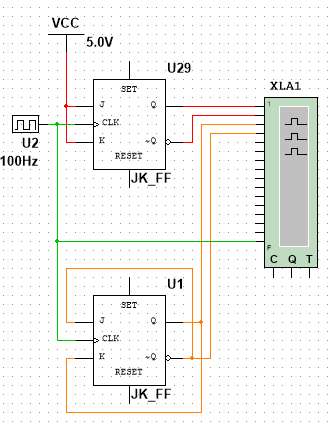
\includegraphics[height=10cm]{reports/img/Z3A_1.png}\\
            \end{center}
            Zadaniem dwójki liczącej jest odtworzenie otrzymanego cyfrowego sygnału zegarowego z dwukrotnie niższą częstotliwością. Pierwszą dwójkę liczącą uzyskałem poprzez podanie stanu wysokiego na wejścia J i K przerzutnika. Tak ustawiony przerzutnik z każdym okresem zegara głównego zamienia stan wyjściowa Q na przeciwny. Zależność tą zilustrować możemy za pomocą poniższego wykresu. 
            
            
            \begin{center}
                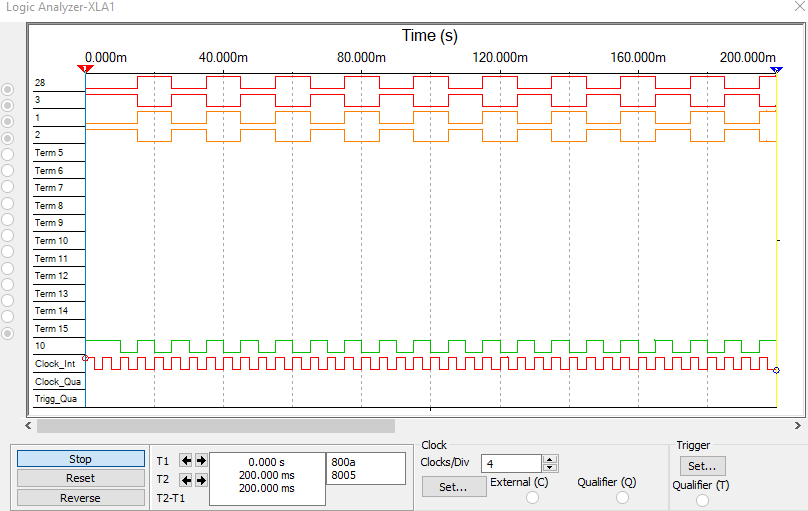
\includegraphics[height=10cm]{reports/img/Z3A_2.png}\\
            \end{center}
            

\end{document}